\chapter{Introduzione}
\label{sec:intro}

\section[Programmazione su GPU]{Programmazione su GPU}

Sin dalla nascita delle prime \gls{CPU}, l'obiettivo principale degli ingegneri è stato quello di aumentane velocità ed efficienza. Sono state sviluppate diverse tecniche per aumentare le prestazioni: come le \textit{\gls{CPU} pipelined}, che permettono di aumentare il throughput delle istruzioni, la \textit{multilevel cache}, per nascondere la latenza della memoria principale rispetto alla velocità di clock del processore, l'\textit{instruction level parallelism} e processori superscalari, per eseguire più istruzioni durante un singolo ciclo di clock.
Quando gli ingegneri si sono accorti che queste metodologie non sarebbero bastate per tenere viva la legge di Moore \cite[]{Moore:law}, si è passati ad un approccio \textit{multi-core}, che ha portato a una nuova forma di parallelismo: parti dell'applicazione possono essere eseguite in contemporanea sui diversi core della stessa \gls{CPU}. L'impatto delle \gls{CPU} multi-core, per accelerare le applicazioni, è stato considerevole, ma il numero limitato di core che possono essere presenti sulla singola unità \gls{CPU} è uno dei maggiori ostacoli che tutt'oggi limita l'ulteriore aumento di prestazioni. In fig. \ref{fig:moore_law} è mostrato come, grazie alla tecnologia multi-core, la legge di Moore può essere ancora considerata valida.

\begin{figure}[ht]
\centering
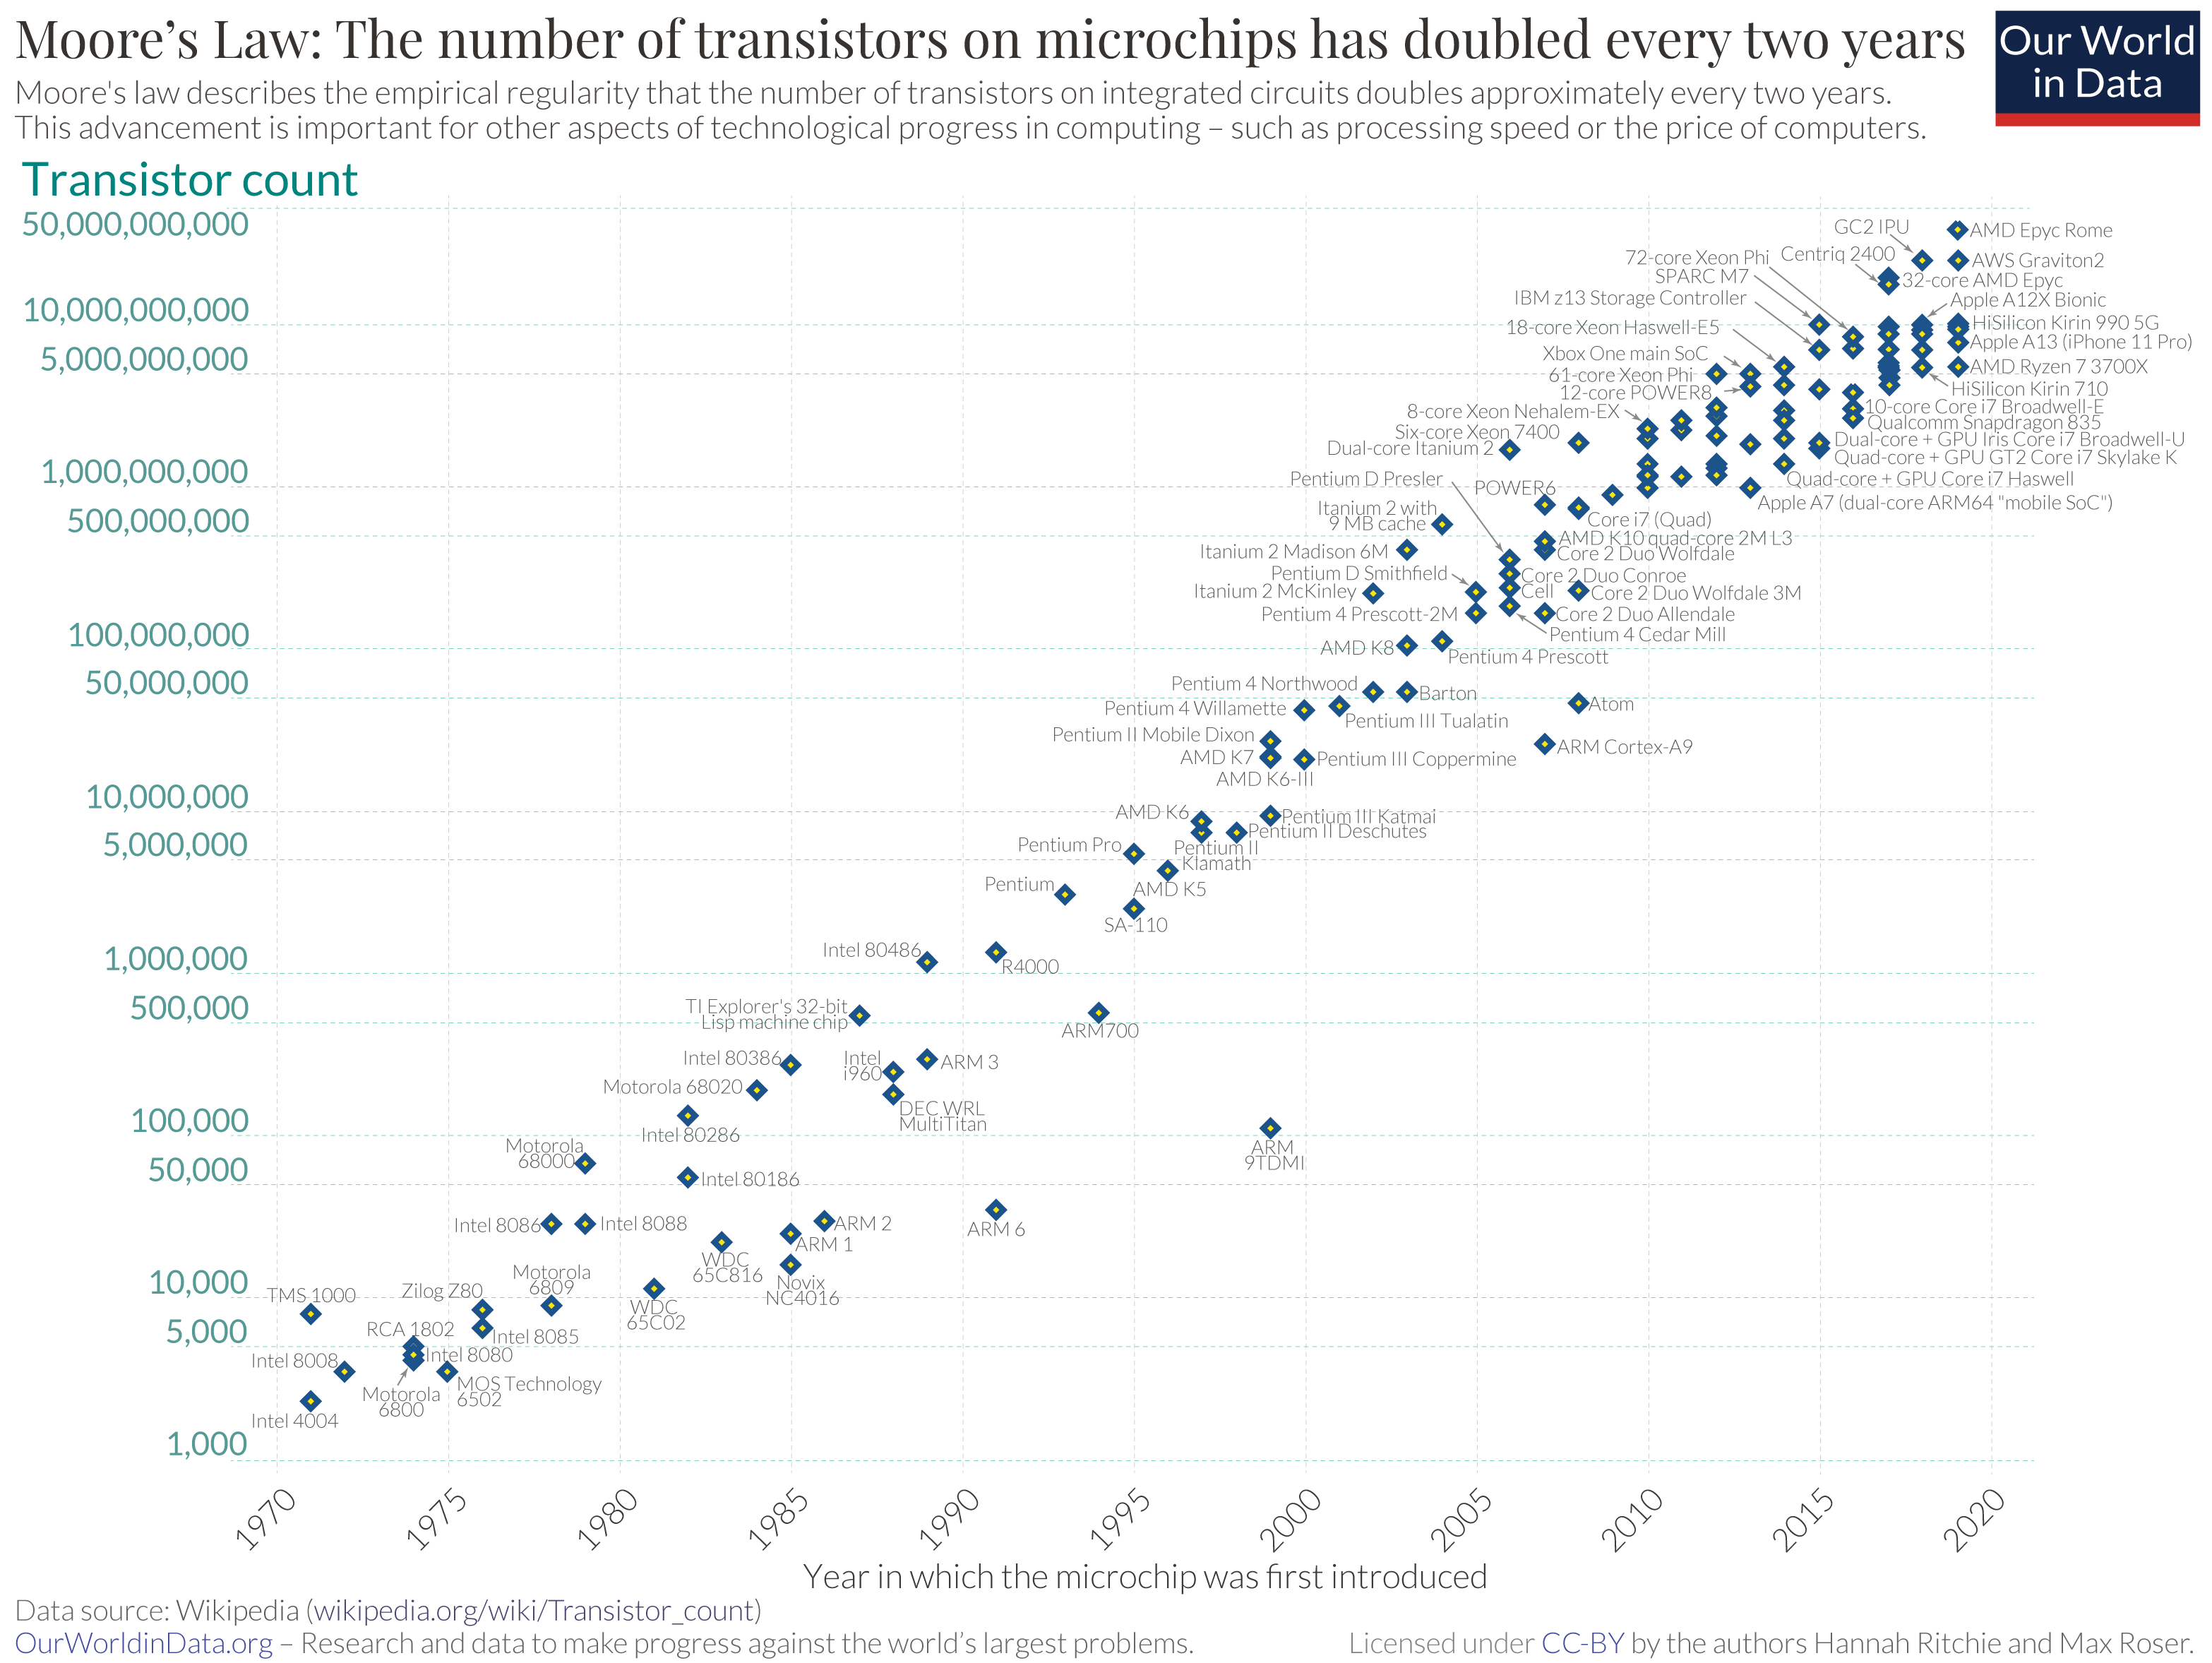
\includegraphics[width=.9\linewidth]{images/chapter1/moore_law.png}
\caption{Legge di Moore [fonte: ourworldindata.org]}
\label{fig:moore_law}
\end{figure}

% GPU

Le \gls{GPU} sono speciali processori, la cui architettura prende a piene mani il concetto di multi-core e lo esalta, al punto da avere tantissimi core, più semplici e lenti dei core \gls{CPU}, ma con un più alto throughput totale.
Originariamente le \gls{GPU} sono state sviluppate per scopi legati all'elaborazione grafica, in particolare, per migliorare la resa delle immagini e la grafica 3D nei videogiochi, nelle applicazioni \gls{CAD} e nei software di modellazione e rendering. In seguito, le esigenze di una grafica sempre più dettagliata e complessa ha portato alla creazione di unità di elaborazione specializzate, con un'architettura che le rende energicamente più efficienti di una \gls{CPU}, per algoritmi che processano grossi blocchi di dati in parallelo. Le \gls{GPU} sono state quindi fruttate anche per scopi diversi dall'elaborazione grafica. Si sono rivelate particolarmente utili per applicazioni scientifiche, \gls{HPC} e tecniche che richiedono elaborazione intensive, come la simulazione di modelli numerici, l'analisi dei dati e il calcolo scientifico. In tempi recenti, le \gls{GPU} vengono impiegate per l'addestramento e l'esecuzione di reti neurali, diventando uno strumento fondamentale per lo sviluppo dell'intelligenza artificiale.

% GPGPU

Quando si parla di \gls{GPGPU} si intende l'utilizzo delle \gls{GPU} per compiti di calcolo generale, rendendole molto più che semplici dispositivi per l'elaborazione grafica. Questo è fondamentale per accelerare algoritmi di calcolo che richiedono enorme quantità di risorse, a patto che la computazione sia parallelizzabile su più processori.
Calcoli che prima richiedevano l'uso di supercomputer, adesso si possono eseguire con una normale \gls{GPU} desktop.
Nel 2011, secondo la lista Top500, che classifica e descrive nel dettaglio i 500 sistemi informatici non distribuiti più potenti al mondo, il Tianhe-1A risultava il secondo supercomputer più potente al mondo. Grazie a un sistema basato sulle \gls{GPU} NVIDIA Tesla M2050 \cite[]{Tianhe-1A:link} il Tianhe-1A è riuscito a raggiungere i 4.7 petaFLOPS di potenza computazionale. Solamente un anno dopo, invece, in vetta alla classifica spiccava il Titan \cite[]{Titan:link}, con un sistema basato sulle più performanti \gls{GPU} NVIDIA Tesla K20X, raggiungendo i 17.59 petaFLOPS di potenza.
Da quell'anno divenne chiaro che le \gls{GPU} sarebbero diventate una componente essenziale nell'\gls{HPC} tanto quanto lo erano nel desktop computing. Dato che il supercomputing è il motore trainante di molte delle tecnologie che vediamo nei processori moderni, si è venuto a creare un circolo virtuoso: la necessità di processori sempre più veloci, per elaborare dataset sempre più grandi, porta l'industria a produrre supercomputer sempre più potenti, tramite i quali si possono progettare processori migliori. Ad oggi, si sta delineando una divisione netta nella produzione di \gls{GPU} per uso desktop e per uso scientifico, i principali produttori, quali AMD, NVIDIA e Intel rilasciano prodotti specificatamente per l'uno o per l'altro segmento di mercato, con lo scopo di soddisfare i diversi requisiti di ogni settore. Da giugno 2023 il supercomputer più veloce al mondo è il Frontier, e con un sistema basato sulle \gls{GPU} Radeon Instinct MI250X riesce a raggiungere i 1.67 exaFLOPS, divenendo il primo exascale supercomputer al mondo \cite[]{Frontier:link}. Grazie all'uso delle \gls{GPU}, si riescono a incrementare le performance dei supercomputer in modo esponenziale, come si può notare in fig. \ref{fig:supercomputer_flops}. L'incremento così repentino delle performance ha portato gli esperti di settore a coniare una nuova legge empirica: la legge di Huang \cite[]{Huang:law}, da Jensen Huang, CEO e co-founder di NVIDIA. La legge enuncia che le performance delle \gls{GPU} ``più che raddoppiano ogni due anni''. In pratica, la legge di Huang è analoga alla legge di Moore, ma applicata alle GPU.

\begin{figure}[ht]
\centering
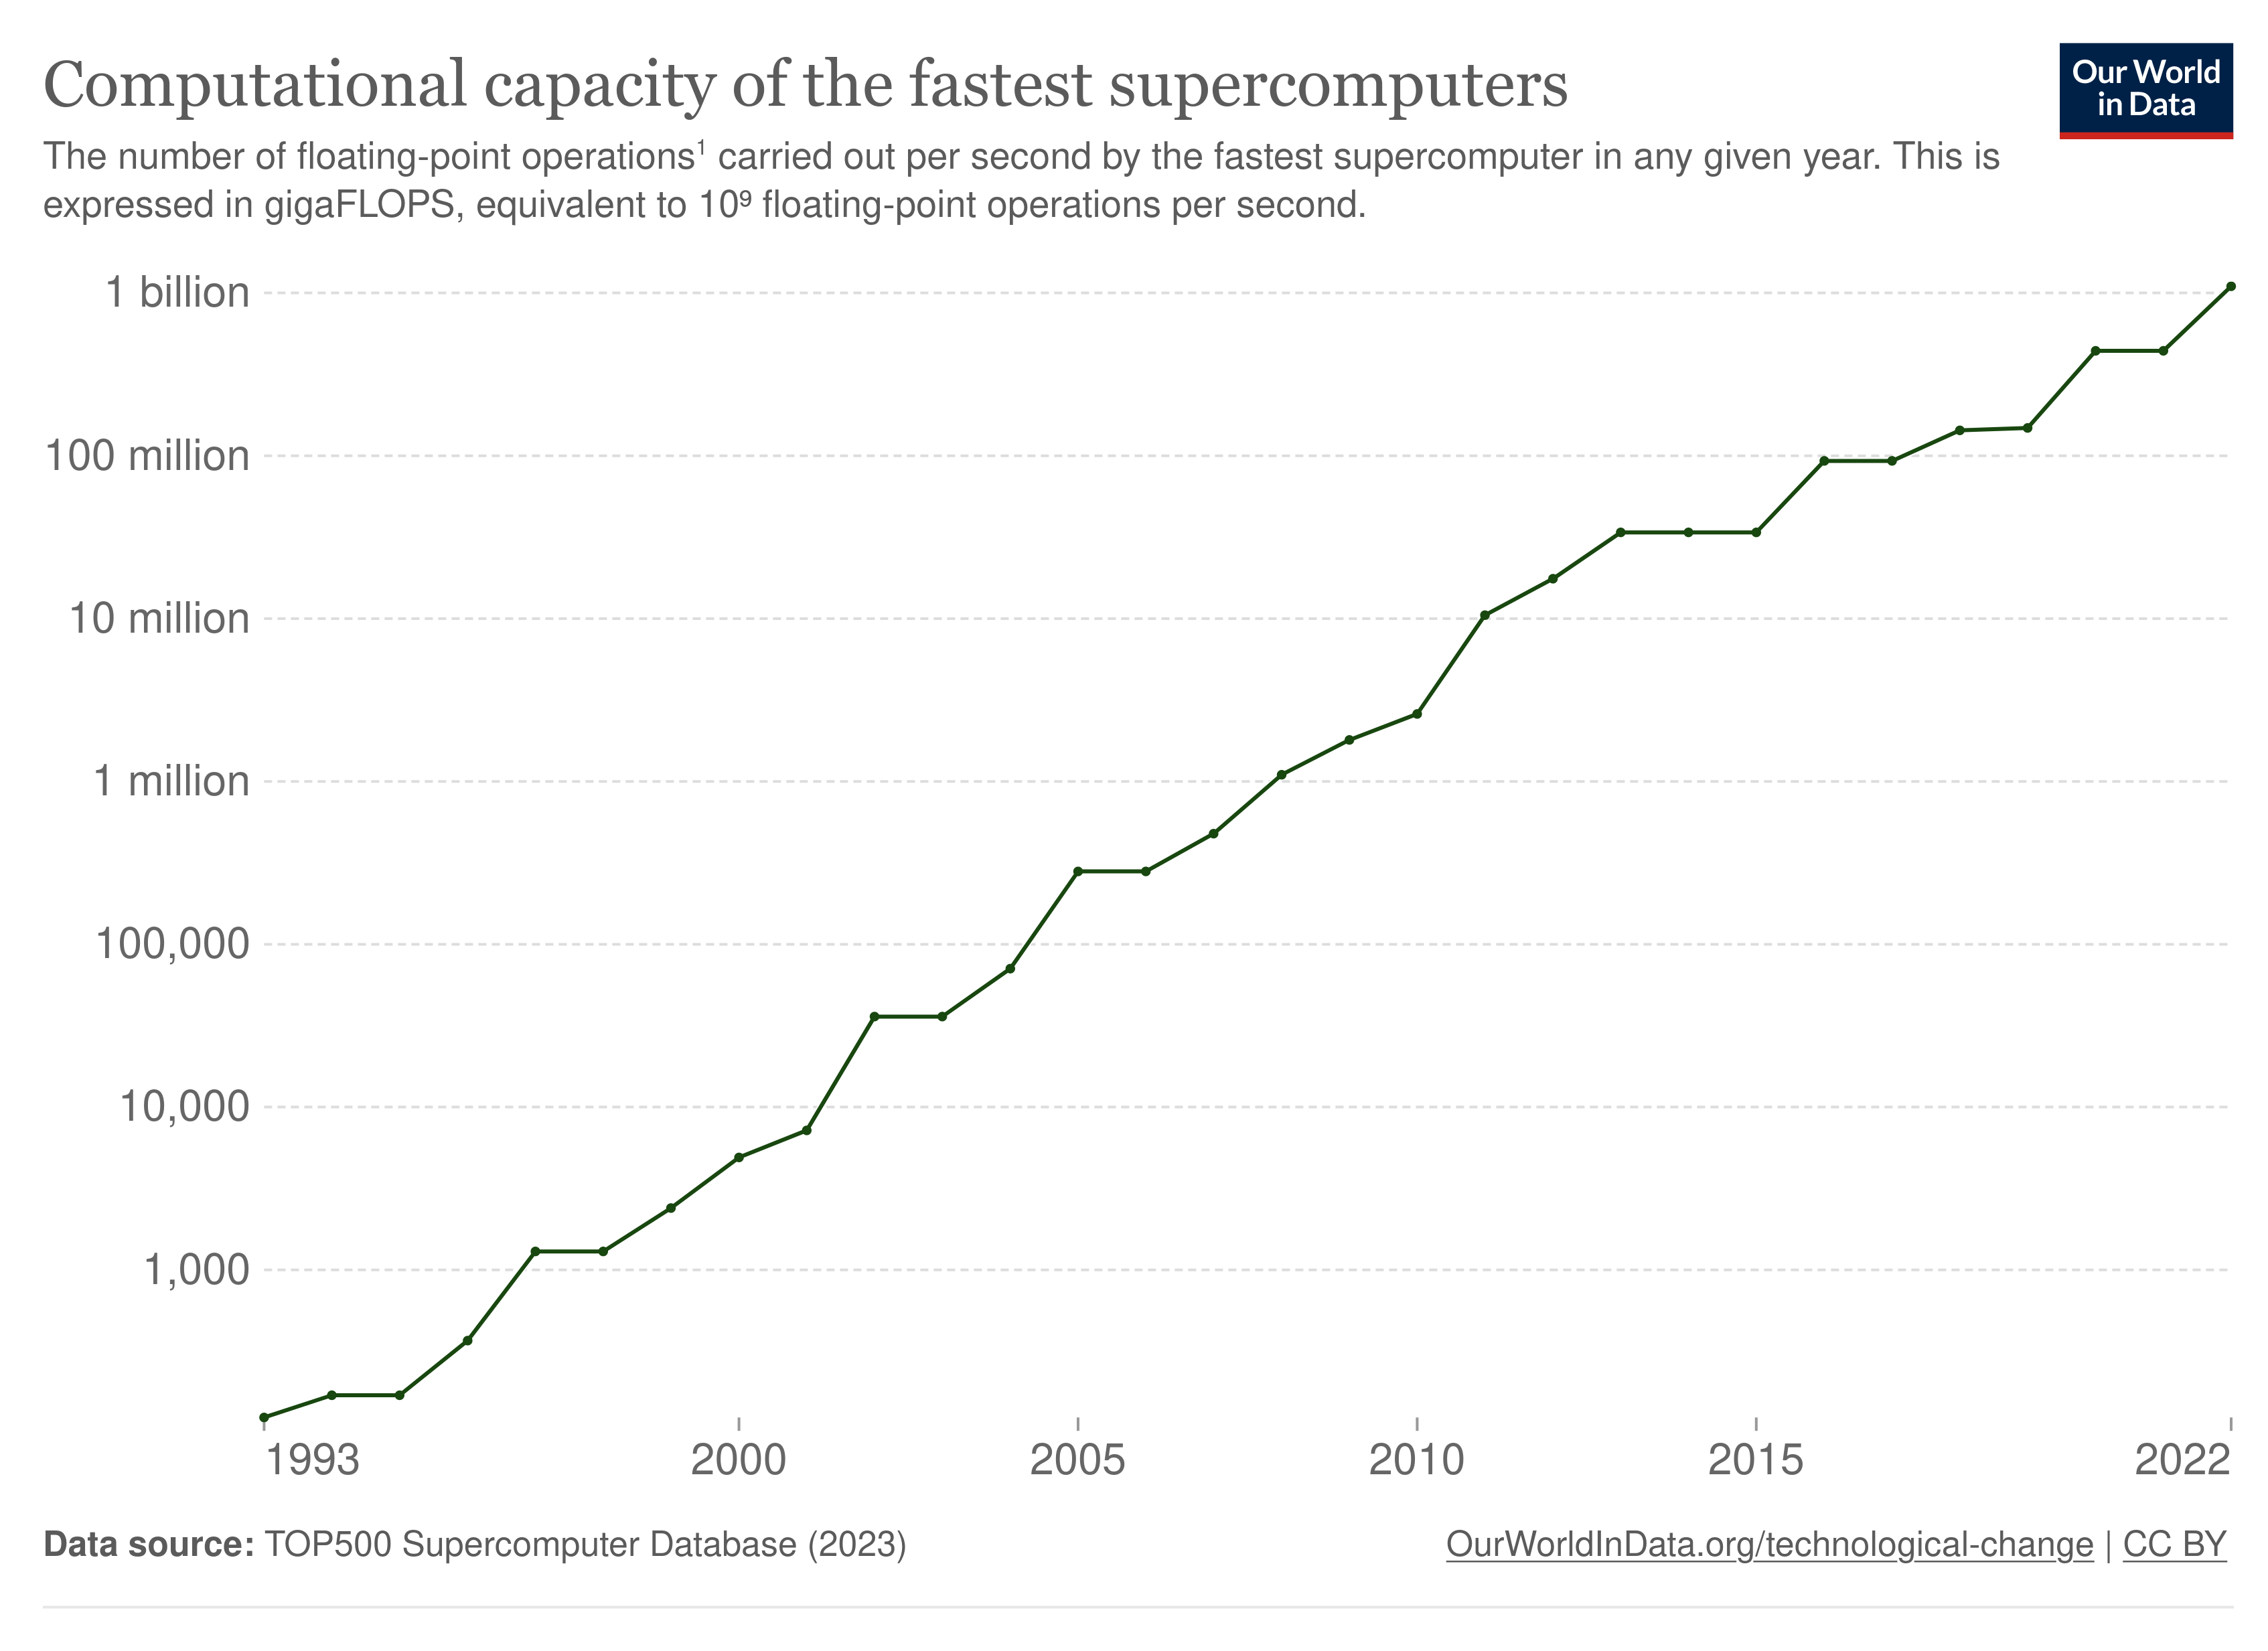
\includegraphics[width=.95\linewidth]{images/chapter1/supercomputer_flops.png}
\caption{Potenza dei supercomputer negli anni [fonte: ourworldindata.org]}
\label{fig:supercomputer_flops}
\end{figure}

%% Librerie GPU programming

Per poter programmare le \gls{GPU} è stato necessario sviluppare delle \gls{API} che garantissero l'esecuzione del programma senza un'esplicita conversione dei dati in formato grafico. Le \gls{API} oggi più utilizzate sono le \gls{CUDA} \gls{API} di NVIDIA \cite[]{NVIDIA:CUDA} e le OpenCL \gls{API} di Khronos Group \cite[]{KG:OpenCL}. Le \gls{API} \gls{CUDA} sfruttano l'omonima architettura delle \gls{GPU} NVIDIA e sono in formato proprietario, mentre le \gls{API} OpenCL, come suggerisce il nome, sono uno standard aperto \textit{royalty-free} e supportano la maggior parte delle architetture \gls{GPU} esistenti. Sebbene queste abbiano prestazioni di molto inferiori rispetto a CUDA, OpenCL è la prima scelta per lo sviluppo di applicazioni multi-piattaforma, proprio per la sua natura open e l'ampio supporto hardware. Nel 2015 Khronos Group annuncia le Vulkan \gls{API} \cite[]{KG:Vulkan} e il formato \gls{SPIR-V} \cite[]{KG:SPIR-V}. Vulkan è una \gls{API} grafica e di calcolo che offre un accesso ad alta efficienza e multi-piattaforma alle \gls{GPU} e \gls{CPU} moderne. Viene utilizzato in una vasta gamma di dispositivi, da PC e console, a telefoni cellulari e piattaforme embedded. Vulkan è stato progettato per sfruttare pesantemente il \textit{multithreading}, permettendo la generazione di carichi di lavoro asincroni da parte di thread multipli della \gls{CPU}, che eseguono il codice sulla \gls{GPU} solo dopo una esplicita sottomissione. Inoltre, la sua natura \textit{close-to-metal} permette un controllo oculato delle risorse della \gls{GPU}: lo sviluppatore è responsabile della sincronizzazione, allocazione di memoria e della sottomissione del lavoro, il che risulta in un minore overhead del driver rispetto a OpenCL. \gls{SPIR-V} è un formato di rappresentazione intermedia per shader, che permette di scrivere il codice una volta e poi compilarlo per diverse architetture, sia \gls{GPU} che \gls{CPU}. Vulkan e \gls{SPIR-V} sono stati sviluppati per essere usati insieme, ma non sono strettamente legati, infatti \gls{SPIR-V} può essere usato anche con OpenCL e OpenGL.

\section[Problema e Contributi]{Problema e Contributi}

L'obiettivo di questo lavoro di tesi è valutare i potenziali vantaggi derivanti dall'utilizzo di Vulkan e Rust per lo sviluppo di applicazioni di computing, rispetto all'approccio tradizionale basato su \gls{CUDA}.
Nonostante Vulkan sia largamente usato nell'industria dei videogiochi, usarlo in ambito computing è una sfida non banale, a causa delle \gls{API} verbose e del controllo meticoloso sulle strutture dati.
Un'idea per ridurre il carico intellettivo per lo sviluppatore, e rendere la \textit{development experience} più fluida e appagante, può essere quella gestire la memoria in modo automatico. Solitamente, quando si parla di gestione automatica della memoria, si fa riferimento a \textit{garbage collector} o contatori di riferimenti. Per quanto valido sia questo approccio, il risultato non sempre è performante e ad alta efficienza, requisito fondamentale in ambito computing. Per mantenere le prestazioni quanto più vicine possibile a un'implementazione \textit{low level}, senza sacrificare l'ergonomicità di un approccio ad alto livello, si è scelto di coniugare i vantaggi del linguaggio Rust, quali, appunto, la gestione automatica della memoria senza strumenti di garbage collections, con quelli che offre Vulkan.

Per poter capire se Vulkan e Rust sono una valida alternativa a \gls{CUDA} per il computing, è necessario rispondere alle seguenti domande:

% bullet points
\begin{itemize}
    \item Qual è il livello di performance che Vulkan riesce a raggiungere rispetto a \gls{CUDA}?
    \item Quanto è difficile sviluppare un'applicazione per il computing in Vulkan?
    \item In un ambiente a microservizi, quanto è facile sviluppare e mantenere un'applicazione Vulkan scritta in Rust?
    \item Qual è il livello di maturità dell'ecosistema Vulkan? E quello di Rust?
\end{itemize}

Per rispondere a queste domande si è agito nel seguente modo:

\begin{itemize}
    \item Si è scelto di implementare algoritmi altamente parallelizzabili su \gls{GPU}, quali la somma di vettori e moltiplicazione di matrici, da usare come banco di prova per comparare le performance di implementazioni in \gls{CUDA} e Vulkan. In particolare, si è preso in considerazione sia il tempo dell'esecuzione dell'algoritmo, che il tempo di trasferimento dei dati in memoria.
    \item Si è implementato gli algoritmi in Vulkan per valutare il potenziale delle sue \gls{API} \textit{close-to-metal} e quanto sia ergonomico sviluppare in Rust. Dato che sviluppare in Vulkan richiede degli step di inizializzazione, quali la creazione di un \textit{logical device}, una \textit{pipeline}, la compilazione del codice dello shader e l'allocazione di memoria, si è usata la libreria Rust Vulkano \cite[]{Rust:Vulkano}, che implementa delle interfacce \textit{safe} all'implementazione standard di Vulkan.
    \item Si è poi reimplementato i medesimi algoritmi in \gls{CUDA}, per comparare sia le performance che il diverso approccio alla scrittura dei kernel, come estensione del linguaggio C++ tramite il compilatore \gls{NVCC} \cite[]{NVIDIA:nvcc}, osservando che \gls{GLSL} \cite[]{KG:GLSL} usato in Vulkan offre più funzioni orientate alla grafica che al computing.
    \item Infine, considerando l'esperienza di sviluppo e i risultati relativi ai benchmark ottenuti, si è sviluppato un microservizio \textit{proof of concept}, che coniuga i vantaggi di Rust in ambito web con quelli di \gls{CUDA} in ambito computing. Si è inoltre valutato anche altri possibili approcci alla soluzione del problema.
\end{itemize}

\newpage

\section[Struttura della tesi]{Struttura della tesi}

L'elaborato è strutturato nei seguenti capitoli:

\begin{itemize}
    \item \textbf{Capitolo 1}: Introduzione e storia delle \gls{GPU} e del \gls{HPC}.
    \item \textbf{Capitolo 2}: Introduzione alla \gls{GPGPU} e alle \gls{API} di programmazione, con particolare attenzione a Vulkan e \gls{CUDA}, e una breve descrizione di Rust.
    \item \textbf{Capitolo 3}: Descrizione del problema, e analisi dei requisiti del progetto finale, con valutazione dei possibili approcci al problema con relativi pro e contro.
    \item \textbf{Capitolo 4}: Descrizione dell'architettura usata per i benchmark e esposizione dei dati raccolti.
    \item \textbf{Capitolo 5}: Analisi dei dati raccolti dai benchmark e considerazioni sullo sviluppo degli applicativi.
    \item \textbf{Capitolo 6}: Implementazione del microservizio e valutazione delle possibili implementazioni future.
    \item \textbf{Capitolo 7}: Conclusioni e considerazioni finali.
\end{itemize}

Il lavoro è stato progettato, sviluppato e testato con il supporto del team di Quantum Computing di Data Reply con sede a Torino.

